% ---------------------------------------------------------------------------
% Falkner-Skan problem geometry.
%
% A uniform stream of speed v_\infty approaches a symmetric wedge of included
% angle \beta\pi.  A laminar boundary layer grows along the wedge face, driven
% by the external velocity v_{1e}(x_1) = C x_1^n with n = \beta / (2 - \beta).
%
% Build:  pdflatex geometry.tex
% (or, from the repository root:  python -m falkner_skan.figures --geometry)
%
% To embed the drawing in a larger document, copy the tikzpicture environment
% and load \usepackage{tikz} plus \usetikzlibrary{arrows.meta, patterns}.
% ---------------------------------------------------------------------------
\documentclass[tikz, border=6pt]{standalone}
\usepackage{amsmath}
\usetikzlibrary{arrows.meta, patterns}

\begin{document}
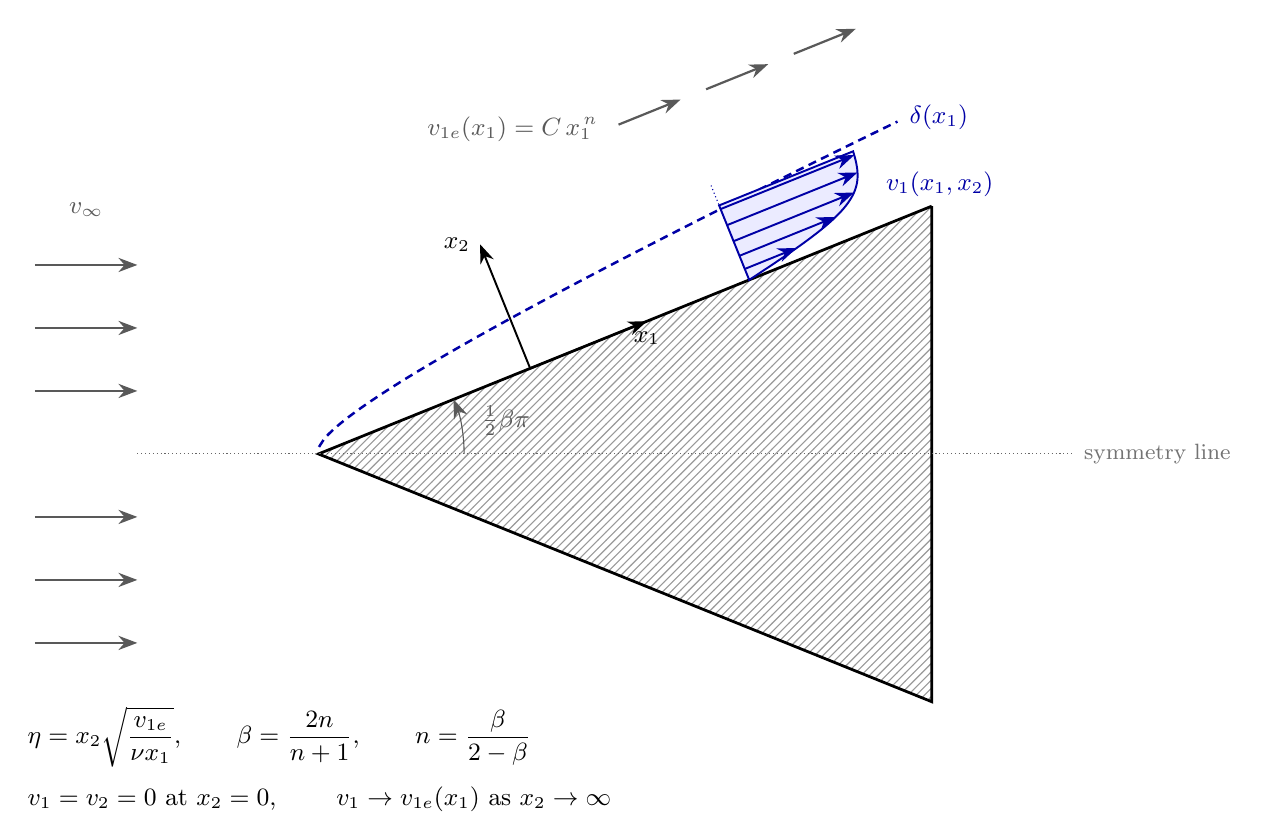
\begin{tikzpicture}[
    >={Stealth[length=2.4mm]},
    wall/.style   = {line width=1pt, black},
    body/.style   = {pattern=north east lines, pattern color=black!40},
    bl/.style     = {line width=0.9pt, blue!65!black, densely dashed},
    prof/.style   = {line width=0.7pt, blue!65!black},
    stream/.style = {line width=0.8pt, black!65, ->},
    axis/.style   = {line width=0.7pt, ->},
    font=\small,
  ]

  % --- wedge half-angle in degrees: half of the included angle \beta\pi -----
  \def\halfangle{22}     % => \beta = 2 x 22/180 = 0.244,  n = 0.139
  \def\len{8.4}          % length of the wedge face that is drawn

  % --- oncoming uniform stream ---------------------------------------------
  \foreach \y in {-2.4, -1.6, -0.8, 0.8, 1.6, 2.4} {
    \draw[stream] (-3.6, \y) -- (-2.3, \y);
  }
  \node[black!65] at (-2.95, 3.1) {$v_\infty$};

  % --- the wedge -----------------------------------------------------------
  \fill[body]  (0,0) -- (\halfangle:\len) -- (-\halfangle:\len) -- cycle;
  \draw[wall]  (\halfangle:\len) -- (0,0) -- (-\halfangle:\len)
               -- (\halfangle:\len);

  % --- symmetry line and the wedge angle -----------------------------------
  \draw[densely dotted, black!60] (-2.3,0) -- (9.6, 0)
    node[anchor=west, black!55, font=\footnotesize] {symmetry line};
  \draw[->, black!65] (1.85,0) arc (0:\halfangle:1.85);
  \node[black!65, anchor=west] at (1.95, 0.42) {$\tfrac{1}{2}\beta\pi$};

  % =========================================================================
  % Everything below is expressed in the wall-aligned frame: x_1 runs along
  % the wedge face from the apex, x_2 is normal to it.
  % =========================================================================
  \begin{scope}[rotate=\halfangle]

    % --- boundary-layer edge,  delta ~ sqrt(x_1) --------------------------
    \draw[bl] plot[domain=0.04:\len, samples=80, smooth]
      (\x, {0.40*sqrt(\x)});
    \node[blue!65!black, anchor=west] at (\len+0.05, 1.20) {$\delta(x_1)$};

    % --- local coordinate axes --------------------------------------------
    \draw[axis] (2.9,0) -- (4.5,0) node[anchor=north] {$x_1$};
    \draw[axis] (2.9,0) -- (2.9,1.7) node[anchor=east] {$x_2$};

    % --- external velocity along the edge of the layer --------------------
    \foreach \x in {5.1, 6.3, 7.5} {
      \draw[stream] (\x, 2.45) -- (\x+0.85, 2.45);
    }
    \node[black!65, anchor=east] at (4.95, 2.45)
      {$v_{1e}(x_1) = C\,x_1^{\,n}$};

    % --- velocity profile at one station ----------------------------------
    \def\xs{5.9}
    \def\dmax{1.02}
    % A tanh profile stands in for f'(\eta): in a sketch the shape is what
    % matters, not the values.
    \draw[prof, fill=blue!8]
      plot[domain=0:\dmax, samples=40, smooth]
        ({\xs + 1.85*tanh(2.70*\x)}, \x)
      -- (\xs, \dmax) -- (\xs, 0) -- cycle;
    \foreach \y in {0.15, 0.33, 0.53, 0.75, 0.97} {
      \draw[prof, ->] (\xs, \y) -- ({\xs + 1.85*tanh(2.70*\y)}, \y);
    }
    \draw[densely dotted, blue!65!black] (\xs, 0) -- (\xs, \dmax+0.30);
    \node[blue!65!black, anchor=west] at (\xs+1.95, 0.52)
      {$v_1(x_1, x_2)$};

  \end{scope}

  % --- statement of the problem, as a caption inside the picture -----------
  \node[anchor=north west, align=left, font=\small, inner sep=0pt]
    at (-3.7, -3.2)
    {$\displaystyle
       \eta = x_2\sqrt{\frac{v_{1e}}{\nu x_1}},
       \qquad \beta = \frac{2n}{n+1},
       \qquad n = \frac{\beta}{2-\beta}$
     \\[6pt]
     $v_1 = v_2 = 0$ at $x_2 = 0$,
     \qquad $v_1 \to v_{1e}(x_1)$ as $x_2 \to \infty$};

\end{tikzpicture}
\end{document}
